\section{Classification}

Classification involves learning an approximation of a function $f(x)$ that maps inputs $x$ to discrete classes $C_k$ (with $k=1,\dots,K$) from a dataset $\mathcal{D}$: 
\[\mathcal{D}=\left\{ \left\langle x,C_k \right\rangle \right\} \implies C_k=f(x)\]
Various approaches to classification include:
\begin{itemize}
    \item \textit{Discriminant function}: modeling a parametric function that directly maps inputs to classes and learning the parameters from the data.
    \item \textit{Probabilistic discriminative approach}: designing a parametric model of $\Pr(C_k\mid\textbf{x})$ and learning the model parameters from the data.
    \item \textit{Probabilistic generative approach}: modeling $\Pr(\textbf{x}\mid C_k)$ and class priors $\Pr(C_k)$, fitting models to the data, and inferring the posterior using Bayes' rule.
\end{itemize}
In linear classification, we will use generalized linear models: 
\[f(\textbf{x},\textbf{w})=f(\textbf{x}^T\textbf{w}+w_0)\]
Here, the function $f(\cdot)$ is not linear in $\textbf{w}$ and partitions the input space into decision regions, with their decision boundaries.
Notably, these decision boundaries are linear functions of $\textbf{x}$ and $\textbf{w}$, expressed as:
\[\textbf{x}^T\textbf{w}+w_0=\text{constant}\]

The labels in a classification problem can be encoded in different ways, depending on the numbers of labels: 
\begin{itemize}
    \item \textit{Two labels}: we can choose between $t \in \{0,1\}$ and $t \in \{-1,1\}$ depending on the specific situation. 
        The first encoding is useful when we need to model probabilities, the second one is preferable for certain algorithms. 
    \item \textit{Multiple lables}: in this scenario we have $K$ labels and the typical encoding is called $1$-of-$K$. 
        Here, $t$ is a vector of length $K$, with a $1$  in the position corresponding to the encoded class.
\end{itemize}

\paragraph*{Two-class problem}
The most general formulation for a discriminant linear function in a two-class linear problem is:
\[f(\textbf{x},\textbf{w})=\begin{cases}
    C_1 \qquad \text{if } \textbf{x}^T\textbf{w}+w_0 \geq 0 \\
    C_2 \qquad \text{otherwise}
\end{cases}\]
From this formulation, we can deduce the following properties:
\begin{itemize}
    \item The decision boundary is $y(\cdot)=\textbf{x}^T\textbf{w}+w_0=0$. 
    \item The decision boundary is orthogonal to $\textbf{w}$. 
    \item The distance of the decision boundary from the origin is $\frac{w_0}{{\left\lVert \textbf{w}\right\rVert}_2 }$.
    \item The distance of the decision boundary from $\textbf{x}$ is $\frac{y(\textbf{x})}{{\left\lVert \textbf{w}\right\rVert}_2 }$.
\end{itemize}
\begin{figure}[H]
    \centering
    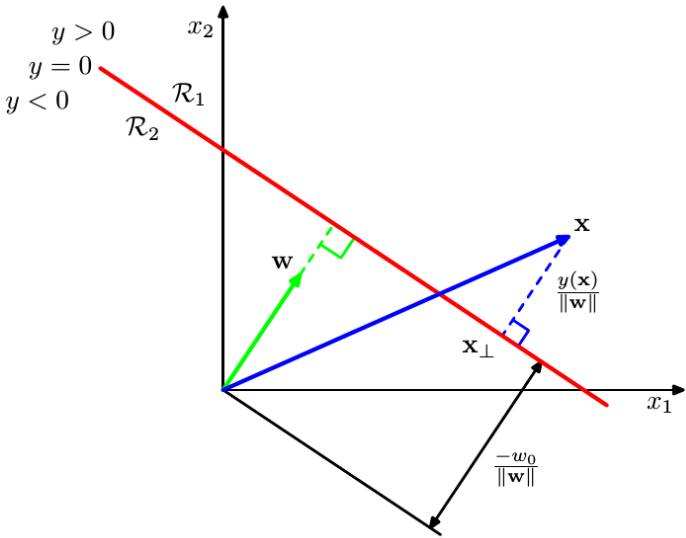
\includegraphics[width=0.35\linewidth]{images/2c.png}
    \caption{Two-class decision problem boundaries}
\end{figure}

\paragraph*{Multiple-class problem}
In multiple class problems with $K$ classes, various encoding methods can be employed:
\begin{itemize}
    \item \textit{One versus the rest}: this approach involves using $K-1$ binary classifiers, where each classifier distinguishes between one class and the rest of the classes.
        However, this method introduces ambiguity since there may be regions mapped to multiple classes.
    \item \textit{One versus one}: this method utilizes $\frac{K(K-1)}{2}$ binary classifiers, where each classifier discriminates between pairs of classes. 
        Similar to the one versus the rest approach, this method also suffers from ambiguity.
    \item \textit{Linear discriminant functions}: one solution to mitigate the ambiguity in multi-class classification is to employ $K$ linear discriminant functions:
        \[y_k(\textbf{x})=\textbf{x}^T\textbf{w}_k+w_{k0} \qquad k=1,\dots,K\]
        In this approach, an input vector $\textbf{x}$ is assigned to class $C_k$ if $y_k>y_j$ for all $j \neq k$. 
        This method ensures that the decision boundaries are singly connected and convex.
\end{itemize}

\paragraph*{Basis functions}
Up to this point, we have focused on models operating within the input space.
However, we can enhance these models by incorporating a fixed set of basis functions $\boldsymbol{\phi}(\textbf{x})$. 
Essentially, this involves applying a non-linear transformation to map the input space into a feature space. 
Consequently, decision boundaries that are linear within the feature space would correspond to nonlinear boundaries within the input space.
This extension enables the application of linear classification models to problems where samples are not linearly separable.

\paragraph*{Ordinary Least Squares}
Let's consider a $K$-class problem using a $1$-of-$K$ encoding for the target. 
Each class is modeled with a linear function:
\[y_k(\textbf{x})=\textbf{x}^T\textbf{w}_k+w_{k0} \qquad k=1,\dots,K\]
In matrix notation, this can be expressed as $\textbf{y}(\textbf{x})=\tilde{\textbf{w}}^T\tilde{\textbf{x}}$. 
Given a dataset $\mathcal{D}=\left\{ \textbf{x}_i, \textbf{t}_i  \right\}$ where $i=1,\dots,N$, we can utilize the Least Squares method to determine the optimal value of $\tilde{\textbf{w}}$, resulting in:
\[\tilde{\textbf{w}}=\left(\tilde{\textbf{x}}^T\tilde{\textbf{x}}\right)\tilde{\textbf{x}}^T\tilde{\textbf{t}}\]
The primary challenge with employing Ordinary Least Squares in classification is that the resulting decision boundaries between regions can vary significantly based on the distribution of the data. 
This method may yield effective or suboptimal boundaries depending on the characteristics of the dataset.

\subsection{Discriminant function approach}
\paragraph*{Perceptron}
To address the issue of poor boundaries, one approach is to utilize a model known as the Perceptron. 
Proposed by Rosenblatt in 1958, the Perceptron is a generalized linear model designed specifically for two-class problems. 
The Perceptron model is defined as:
\[f(\textbf{x},\textbf{w})=\begin{cases}
    +1 \qquad \text{if } \textbf{x}^T\textbf{w}+w_0 \geq 0 \\
    -1 \qquad \text{otherwise}
\end{cases}\]
The Perceptron algorithm aims to determine a decision surface, also known as a separating hyperplane, by minimizing the distance of misclassified samples to the boundary. 
This minimization of the loss function can be achieved using stochastic gradient descent.
Although simpler loss functions could theoretically be used, they are often more complex to minimize in practice. 

The Perceptron loss function is expressed as:
\[\mathcal{L}_P(\textbf{w})=-\sum_{n \in \mathcal{M}}\textbf{w}^T\textbf{x}_nt_n\]
Here, correctly classified samples do not contribute to $\mathcal{L}_P$. 

Minimizing $\mathcal{L}_P$ is achieved using stochastic gradient descent:
\[\textbf{w}^{(k+1)}=\textbf{w}^{(k)}+\alpha\textbf{x}_nt_n\]
Since the scale of $\textbf{w}$ does not affect the Perceptron function, the learning rate $\alpha$ is often set to $1$. 
The Perceptron algorithm takes a dataset $\mathcal{D}=\left\{ \textbf{x}_i,\textbf{t}_i  \right\}$ where $i=1,\dots,N$. 
\begin{algorithm}[H]
    \caption{Perceptron}
        \begin{algorithmic}[1]
            \State Initialize $\textbf{w}_0$
            \State $k = 0$
            \Repeat
                \State $k = k+1$
                \State $n = k \mod N$
                \If{$\hat{t}_n \neq t_n$}
                    \State $\textbf{w}_{k+1} = \textbf{w}_k + \textbf{x}_nt_n$
                \EndIf
            \Until{convergence}
        \end{algorithmic}
\end{algorithm}
\begin{theorem}[Perceptron convergence]
    If the training dataset is linearly separable in the feature space, then the Perceptron learning algorithm is guaranteed to find an exact solution in a finite number of steps.
\end{theorem}
Several steps may be necessary, making it challenging to distinguish between non-separable problems and slowly converging ones. 
If multiple solutions exist, the one obtained by the algorithm depends on the order of the elements in the dataset.

\paragraph*{K-Nearest Neighbors}
The $K$-Nearest Neighbors algorithm, specifically the 1-Nearest Neighbors variant, follows a discriminative approach by using the proximity of points in the feature space to make predictions for new data points. 
The core idea is to find the closest neighbors to predict the target label of an unseen data point.

Given a dataset $\mathcal{D}=\{(x_n,t_n)\}_{i=1}^M$ and a new data point $\mathbf{x}_q$, 1-NN predicts the target by finding the nearest neighbor according to the Euclidean distance:
\[i_1\in\argmin_{n\in\{1,\dots,N\}}{\left\lVert \mathbf{x}_q- \mathbf{x}_n\right\rVert}_2 \]
KNN works effectively for both regression and classification tasks, and it requires no explicit training phase; the model learns by simply querying the dataset at prediction time.

For $K > 1$, combining the targets from multiple neighbors depends on the type of task:
\begin{itemize}
    \item \textit{Classification}: predict the most frequent class among the $K$-Nearest Neighbors, with a tie-breaking rule if needed.
    \item \textit{Regression}: predict the average target value among the $K$-Nearest Neighbors.
\end{itemize}
This approach can easily handle multiple classes without modification. 
In multi-class classification, the target is the mode class of the neighbors, while in multi-class regression, it is the average target value.

Note that this algorithm needs to have all the dataset stored in main memory and it is non parametric since we do not have explicit parameters to compute. 
Higher values for $k$ reduces the variance.

\subsection{Probabilistic discriminative approach}
In a discriminative approach, we model the conditioned class probability directly:
\[\Pr(C_1\mid \boldsymbol{\phi})=\dfrac{1}{1+e^{-\textbf{w}^T\boldsymbol{\phi}}}=\sigma(\textbf{w}^T\boldsymbol{\phi})\]
This model is commonly referred to as logistic regression (generalized linear model).

\paragraph*{Maximum Likelihood}
Given a dataset $\mathcal{D}=\left\{ \textbf{x}_i,t_i \right\}$, where $i=1,\dots,N$ and $t_i \in \{0,1\}$, we aim to maximize the likelihood.
We model the likelihood of a single sample using a Bernoulli distribution, employing the logistic regression model for conditioned class probability:
\[\Pr(t_n\mid\textbf{x}_n,\textbf{w})=y_n^{t_n}{\left( 1-y_n \right)}^{1-t_n} \qquad y_n=\sigma(\textbf{w}^T\boldsymbol{\phi}_n)\]
Assuming independent sampling of data in $\mathcal{D}$, we have:
\[\Pr(\textbf{t}\mid\textbf{x},\textbf{w})=\prod_{n=1}^N y_n^{t_n}{\left( 1-y_n \right)}^{(1-t_n)} \qquad y_n=\sigma(\textbf{w}^T\boldsymbol{\phi}_n)\]
The negative log-likelihood (also known as cross-entropy error function) serves as a convenient loss function to minimize:
\[\mathcal{L}(\textbf{w})=-\ln \Pr(\textbf{t}\mid\textbf{X},\textbf{w})=-\sum_{n=1}^N \left( t_n\ln y_n +(1-t_n) \ln (1-y_n) \right)\]
The derivative of the loss function yields the gradient of the loss function:
\[\dfrac{\partial\mathcal{L}(\textbf{w})}{\partial\mathbf{w}}=\sum_{n=1}^N\left( y_n-t_n \right) \boldsymbol{\phi}_n\]
Due to the nonlinearity of the logistic regression function, a closed-form solution is not feasible. 
Nevertheless, the error function is convex, allowing for gradient-based optimization (online gradient descent).
The convergence is asymtotically guaranteed, also in case of non linearly separable elements. 

\paragraph*{Multi class logistic regression}
In multi class problems, $\Pr(C_k\mid\boldsymbol{\phi})$ is modeled by applying a softmax transformation to the output of $K$ linear functions (one for each class):
\[\Pr(C_k\mid\boldsymbol{\phi})=\dfrac{e^{\textbf{w}_k^T\boldsymbol{\phi}}}{\sum_j e^{\textbf{w}_j^T\boldsymbol{\phi}}}\]
Similar to the two-class logistic regression and assuming $1$-of-$K$  encoding for the target, we compute the likelihood as:
\[\Pr(\textbf{t}\mid\boldsymbol{\Phi},\textbf{w}_1,\dots,\textbf{w}_K)=\prod_{n=1}^N \left( \prod_{k=1}^K \Pr{(C_k\mid\boldsymbol{\phi}_n)}^{t_n k} \right)=\prod_{n=1}^N \left( \prod_{k=1}^K y^{t_n k}_{nk} \right)\]
As in the two-class problem, we minimize the cross-entropy error function:
\[L(\textbf{w}_1,\dots,\textbf{w}_K)=-\ln \Pr(\textbf{t}\mid\boldsymbol{\Phi},\textbf{w}_1,\dots,\textbf{w}_K)=-\sum_{n=1}^N \left(\sum_{k=1}^K t_{nk}\ln y_{nk} \right)\]
Then, we compute the gradient for each weight vector:
\[\dfrac{\partial\mathcal{L}_{\textbf{w}_j}(\textbf{w}_1,\dots,\textbf{w}_K)}{\partial\mathbf{w}} =\sum_{n=1}^N\left( y_{nj}-t_{nj} \right) \boldsymbol{\phi}_n\]
Replacing the logistic function with a step function in logistic regression yields the same updating rule as the Perceptron algorithm.

\subsection{Probabilistic generative approach}
The primary probabilistic generative model for classification is known as Naïve Bayes, which relies on a simplifying assumption known as the Naïve or conditional independence assumption. 
This assumption states that, given a class label $C_k$, the features $x_i$ in the input vector $\mathbf{x}$ are conditionally independent of one another.
Under this assumption, the probability of class given an input is expressed as: 
\[\Pr(C_k\mid\mathbf{x})=\Pr(C_k)\prod_{i=1}^M\Pr(x_j\mid C_k)\]
In Naïve Bayes classification, our goal is to predict the most likely class $y(\mathbf{x})$ for a given input $\mathbf{x}$ by maximizing the posterior probability:
\[y(\mathbf{x})=\argmax_k\Pr(C_k)\prod_{i=1}^M\Pr(x_j\mid C_k)\]
To fit a Naïve Bayes model, we typically use a logarithmic transformation of the posterior probability, resulting in a log-likelihood function that we maximize. 
This optimization is performed through Maximum Likelihood estimation (MLE), where both the class prior and feature likelihoods are directly estimated from the data.

It is important to note that, despite its name, Naïve Bayes is not a Bayesian method. 
In Bayesian analysis, priors are updated with new evidence. 
Here, however, we estimate priors directly from the data without subsequent updates.

Naïve Bayes, as a generative model, allows us to generate synthetic data resembling the original dataset. 
The process to generate a new sample is as follows:
\begin{enumerate}
    \item Select a class $C_{\hat{k}}$ according to the estimated multinomial prior distribution with parameters $\hat{\Pr}(C_1),\dots,\hat{\Pr}(C_K)$.
    \item For each feature $j$, draw a sample $x_j$ from the distribution $\mathcal{N}(\hat{\mu}_{j\hat{k}},\hat{\sigma}^2_{j\hat{k}})$
    \item Repeat this process to generate additional samples as needed.
\end{enumerate}

\subsection{Model evaluation}
To assess the performance of a classifier, we can use a confusion matrix. 
This matrix provides a summary of the number of correctly classified and misclassified samples, offering insights into how well the model distinguishes between classes.
\begin{table}[H]
    \centering
    \begin{tabular}{|c|c|c|}
        \hline
        & \textbf{Actual Class: 1} & \textbf{Actual Class: 0} \\ \hline
        \textbf{Predicted Class: 1} & TP & FP \\ \hline
        \textbf{Predicted Class: 0} & FN & TN \\ \hline
    \end{tabular}
\end{table}
Using the values from the confusion matrix, we can calculate various performance metrics:
\begin{itemize}
    \item \textit{Accuracy}: the fraction of total samples that are correctly classified. 
        This is a general measure of the classifier's performance over the entire dataset. 
        \[\text{Accuracy}=\dfrac{\text{TP}+\text{TN}}{N}\]
    \item \textit{Precision}: the fraction of samples correctly classified as positive out of all samples predicted as positive. 
        Precision indicates how many of the predicted positive samples are actually positive.
        \[\text{Precision}=\dfrac{\text{TP}}{\text{TP}+\text{FP}}\]
    \item \textit{Recall}: the fraction of actual positive samples that are correctly classified. 
        Recall measures the model's ability to identify positive samples from the dataset.
        \[\text{Recall}=\dfrac{\text{TP}}{\text{TP}+\text{FN}}\]
    \item \textit{F1 score}: the harmonic mean of precision and recall, providing a single metric that balances both. 
        The F1 score is particularly useful when you need to find an equilibrium between precision and recall.
         \[\text{F1}=2\dfrac{\text{Precision}\cdot\text{Recall}}{\text{Precision}+\text{Recall}}\]
\end{itemize}
Higher values for these metrics generally indicate better model performance.
These measures are not symmetric; they depend on the choice of the positive class. 
In some applications, you may switch the positive class to obtain metrics that better reflect the classifier's predictive power in that context.